\section{Simulação}
\label{simulacao}

Nesta seção serão abordado os detalhes utilizados na simulação. A seção
\ref{sec:redesSociais} 
descreve como a rede social que constava no dataset utilizada foi
simulada. A seção \ref{sec:codeRede} descreve o modelo de codificação em
rede utilizado.

\subsection{Redes Sociais} \label{sec:redesSociais}

Cada um dos participantes do experimento (93 participantes) possuía um
programa em seu celular que registrava diversas informações, dentre elas
os IDs únicos de celulares identificados. Essas informações eram
registradas a cada 5 minutos (apesar de que na prática não era tão
regular assim, como será discutido posteriormente). No período em que
consideramos em nosso experimento (1 semana) apenas 73 dos 93 usuários
foram considerados. Isso aconteceu pelo fato de considerarmos apenas os
usuários que estavam participando efetivamente do experimento naquele
tempo.

\begin{figure}[ht]
\centering
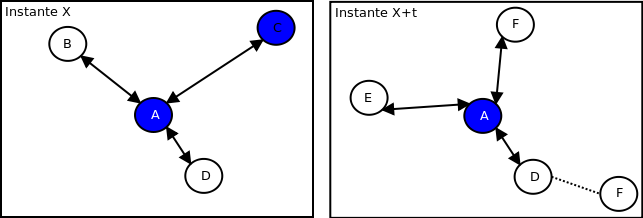
\includegraphics[width=0.7\textwidth]{img/diagramas/redeSocial.png}
\caption{Diagrama que ilustra a dinamicidade da rede considerada na
simulação}
\label{fig:diagramaRedeSocial}
\end{figure}


A Figura \ref{fig:diagramaRedeSocial} ilustra a dinamicidade da rede
considerada na simulação. Para realizar uma simulação mais próxima da
realidade foi preciso realizar uma alteração na estrutura de
funcionamento do simulador utilizado (Sinalgo). Para isso a cada 5
minutos a topologia considerada é alterada. Essa é uma tarefa
computacionalmente cara, sendo um dos motivos que optamos por simular
apenas 1 semana do log. 

O dataset não fornece uma visão completa da rede. Na Figura
\ref{fig:diagramaRedeSocial} os círculos azuis representam usuários
participantes do experimento. Todos os outros círculos representam
usuários não participantes do experimento. Possuímos, através do
dataset, uma visão completa de todos os contatos identificados pelos
participantes do experimento. No entanto, como está representado nessa
figura, não é possível identificar os nodos que entraram em contato
apenas com nodos não participantes do experimento. Essa situação é
ilustrada no contato entre os nodos D e F. De certa forma, como ficará
mais claro posteriormente, essa situação é uma vantagem para o algoritmo
Epidêmico, quando comparado com nosso algoritmo proposto (SocialRoute).


\subsection{Codificação em Rede}\label{sec:codeRede}

Na simulação utilizamos a técnica Random Linear Network Coding (rede
aleatória de codificação). Random Linear Network Coding se baseia em
utilizar códigos aleatórios para transmissão de mensagens codificadas na
rede. Essa técnica foi originalmente proposta em \cite{Ho03thebenefits}.
Na rede aleatória de codificação, os nós da rede, de forma independente,
escolhem aleatoriamente mapeamentos lineares de entrada e saída. O efeito
da rede é a transferência de uma matriz de fontes para os receptores.
Para recuperar os símbolos (ou informações provenientes da origem) nos
receptores, é necessário ter graus de liberdade suficiente - uma matriz
invertível dos coeficientes de todos os nós. Nós receptores podem
decodificar caso eles recebam tantas combinações lineares independentes
como o número de processos (pacotes ou informações originais) da origem.

A Figura \ref{figNetcodingDiagram} ilustra o procedimento utilizado para
a codificação e decodificação dos pacotes transmitidos. Primeiramente a
fonte (ou remetente), envia a informação original ao seus vizinhos. Os
vizinhos, com o auxílio de um vetor aleatório, realiza uma codificação
na informação (o tamanho do vetor aleatório é escolhido baseado no
tamanho do pacote recebido). Em seguida esse pacote codificado é
transmitido a todos os seus vizinhos. Junto com a informação codificada
é transmitido o vetor utilizado para gerar essa codificação. Caso um
nodo receba uma informação codificada e não é o destinatário (ou seja, não
irá realizar o processo de decodificação), ele poderá codificar essa
informação novamente, caso ele tenha em seu poder mais de 1 pacote
codificado recebido e não transmitido. Para realizar esse procedimento é
escolhido um novo vetor aleatoriamente, e é realizado o mesmo
procedimento de codificação com esse novo vetor. Porém, o vetor de
codificação repassado aos vizinhos é o novo vetor escolhido,
multiplicado pelo vetor utilizado para a codificação da informação
recebida.


\begin{figure}[ht]
\centering
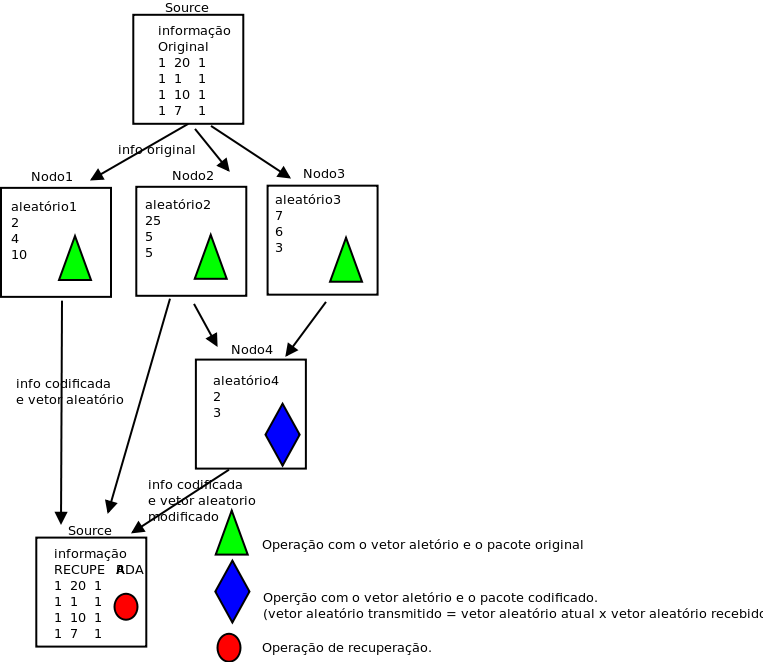
\includegraphics[width=.9\textwidth]{img/diagramas/netCodingDiagram.png}
\caption{Diagrama que ilustra a dinamicidade da rede considerada na
simulação}
\label{figNetcodingDiagram}
\end{figure}

Cada nodo na simulação espera um período de 500ms antes de codificar a
informação. A expectativa dessa espera é que mais pacotes cheguem para
que sejam codificados em apenas um pacote.


\subsection{Algoritmos}\label{algoritmos}

Nas simulações realizadas foram considerados dois algoritmos. O clássico
algoritmo Epidêmico e um algoritmo proposto neste trabalho chamado
SocialRoute. 

Epidêmico: O algoritmo Epidêmico é bastante simples. Cada nodo que
recebe uma mensagem repassa a seus vizinhos (broadcast), caso algum de
seus vizinhos ainda não possui essa informação. 

SocialRoute: Nesse algoritmo, cada nodo somente repassa a informação
caso o nodo atual seja amigo do destinatário, ou caso algum dos vizinhos
do nodo atual sejam amigos do destinatário da mensagem.

\subsection{Parâmetros}

Foram simulados 1666 nodos. Esses nodos representam os usuários
monitorados no experimento realizado pelo MIT Media Lab, e todos os
usuários que o celular dessas pessoas identificaram (através de
bluetooth).

Consideramos uma simulação assíncrona. O simulador utilizado possui
um desempenho consideravelmente melhor ao operar dessa forma. Isso
implica que os nodos não se movimentam na simulação. Mas como
descrito anteriormente, ao mudar a cada 5 minutos a topologia da
rede, captura-se o mesmo efeito de movimentação dos nodos. 

Para simular interferência na comunicação foi utilizado o modelo
SINR. Nesse modelo utilizamos os seguintes valores: $\alpha$ (alpha)
= 2 e $\beta$ (beta) = 0.019.


\subsection{Período considerado}

Como descrito anteriormente o período total do dataset considerado
foi de aproximadamente 9 meses. No entanto em nosso simulador
consideramos um período de 1 semana desse dataset, por duas razões.
A primeira é que nem todos os usuários participantes do experimento,
que resultou no dataset, permaneceram no experimento durante todo o
período de 9 meses. O período do dataset que contêm o maior número
de usuários (participantes do experimento) simultâneos foi o mês de
outubro. O segundo motivo está relacionado ao desempenho da
simulação. Simular os 9 meses do dataset é computacionalmente muito
caro. 

